\documentclass[10pt,twocolumn]{scrartcl}

\usepackage[utf8]{inputenc}
\usepackage[T1]{fontenc}
\usepackage[ngerman]{babel}

\usepackage{amsmath}
\usepackage{amssymb}

\usepackage{graphicx}
\usepackage{tabularx}

\setlength{\parindent}{0cm}
\setlength{\parskip}{3mm}
\setlength{\textheight}{23.8cm}
\setlength{\headheight}{1cm}
\setlength{\topmargin}{-10mm}

\setlength{\oddsidemargin}{0cm}
\setlength{\evensidemargin}{0cm}
\setlength{\textwidth}{16cm}
\setlength{\columnsep}{8mm}

\usepackage{multicol}
\usepackage{colortbl}
\usepackage{xcolor}
\definecolor{grau}{gray}{0.95}
\definecolor{dunkelgrau}{gray}{0.85}

\usepackage[normal]{caption}

\setlength{\parindent}{5mm}
\setlength{\parskip}{0mm}

\usepackage{float}
\restylefloat{figure}

\renewcommand{\topfraction}{0.75}
\renewcommand{\textfraction}{0.2}

%###########################################################
% custom
\newcommand{\TITLE}{Evaluation von Intervallschätzungen und Paramtertests\\ am Beispiel des Buffonschen Nadelproblems}
\newcommand{\AUTHORS}{Lukas Rosenbach\\ David Lennart Risch}

\usepackage[
hidelinks,
linktoc=all
]{hyperref}

\usepackage[list=false, font=large, labelfont=bf,
labelformat=brace, position=top, belowskip=0mm, skip=0mm]{subcaption}

\clubpenalty = 10000
\widowpenalty = 10000
\displaywidowpenalty = 10000
%###########################################################

%###########################################################
% die Sachen mit der Kopfzeile
\usepackage{lastpage}
\usepackage{fancyhdr}
\fancyhf{} % leere alle Felder
\fancyhead[R]{\footnotesize \AUTHORS}
\fancyhead[L]{\footnotesize \TITLE} % Titel des Aufsatzes
\fancyfoot[C]{\footnotesize \thepage/\pageref{LastPage}}
% \fancyfoot[C]{\footnotesize \thepage}
\renewcommand{\headrulewidth}{0.4pt} % obere Trennlinie
\pagestyle{fancy}
%###########################################################

\newcommand{\ownsection}[1]{\begin{center}\LARGE\textbf#1\end{center}}

\begin{document}

\twocolumn[
\ownsection{\TITLE}

\begin{center}
\AUTHORS \\
Mannheim, Juni 2020
\end{center}
\vspace*{5mm}
]

\section*{Abstract}

\section*{Einleitung}

\section{Buffonsches Nadelproblem}
	\label{chap_buffon_needle}
	Bei dem Buffonschen Nadelproblem, das erstmals von Buffon im Jahr 1733 behandelt wurde, geht es um die Wahrscheinlichkeit, dass eine Nadel, die auf eine Fläche mit parallelen Linien gleichen Abstands geworfen wird, eine Linie schneidet.
	
	Dieses Experiment beinhaltet eine Nadel der Länge $l$, die in einem Winkel $\theta$ auf eine Fläche mit parallelen Linien mit dem Abstand $d$ fällt. Für eine kurze Nadel, also $l < d$, lässt sich die Wahrscheinlichkeit wie folgt berechnen: \cite{MathWorld}

	\begin{align}
		P(x) &= \frac{1}{2\pi}\int_{0}^{2\pi}\frac{l|\cos{\theta}|}{d}d\theta \\ \nonumber
		&= \frac{l}{2 \pi d} 4 \int_{0}^{\pi/2}\cos{\theta}d\theta\\ \nonumber
		&= \frac{2l}{\pi d}\\ \nonumber
		&= \frac{2x}{\pi} \nonumber .
	\end{align}
	
	Für einen Linienabstand von $d=2l$ vereinfacht sich die Formel zu
	
	\begin{align}
		P &= \frac{2l}{\pi d}\\ \nonumber
		&= \frac{2l}{\pi (2l)}\\ \nonumber
		&= \frac{1}{\pi} \nonumber .
	\end{align}
	
	Somit ist es möglich durch viele Durchführungen den Wert von Pi mit dem Buffonschen Nadelexperiment anzunähern (Monte-Carlo-Simulation).

\section{Implementierung des Experiments}
	Das Buffonsche Nadelproblem wurde als Python\cite{Python} Programm implementiert, um es mit einer großen Stichprobenzahl statistisch auswerten zu können. Die so erstellten Daten werden von anderen Modulen des Programms verwendet.

	\subsection*{Die Simulation}
		\label{chap_sim_results}
		Im ersten Schritt werden mehrere Nadelwürfe simuliert. Hier muss die Nadellänge, die Breite zwischen den Linien, die Anzahl der Linien und die Höhe des Feldes angegeben. Die Linien verlaufen in der Simulation vertikal. Rechts und links sind die Linien einen halben Linienabstand vom Rand des Feldes entfernt. So kann man gedanklich das Feld am rechten Rand wieder mit dem Linken Rand fortsetzen und erhält ein unendliches Feld. Dann wird für n Nadeln jeweils eine zufällige Position auf dem Feld und ein zufälliger Winkel berechnet. Diese Werte werden dann in einem Ergebnis gespeichert, zusätzlich wird gezählt wie viele Nadeln eine Linie schneiden.

		\begin{figure}[htb]
			\centering
			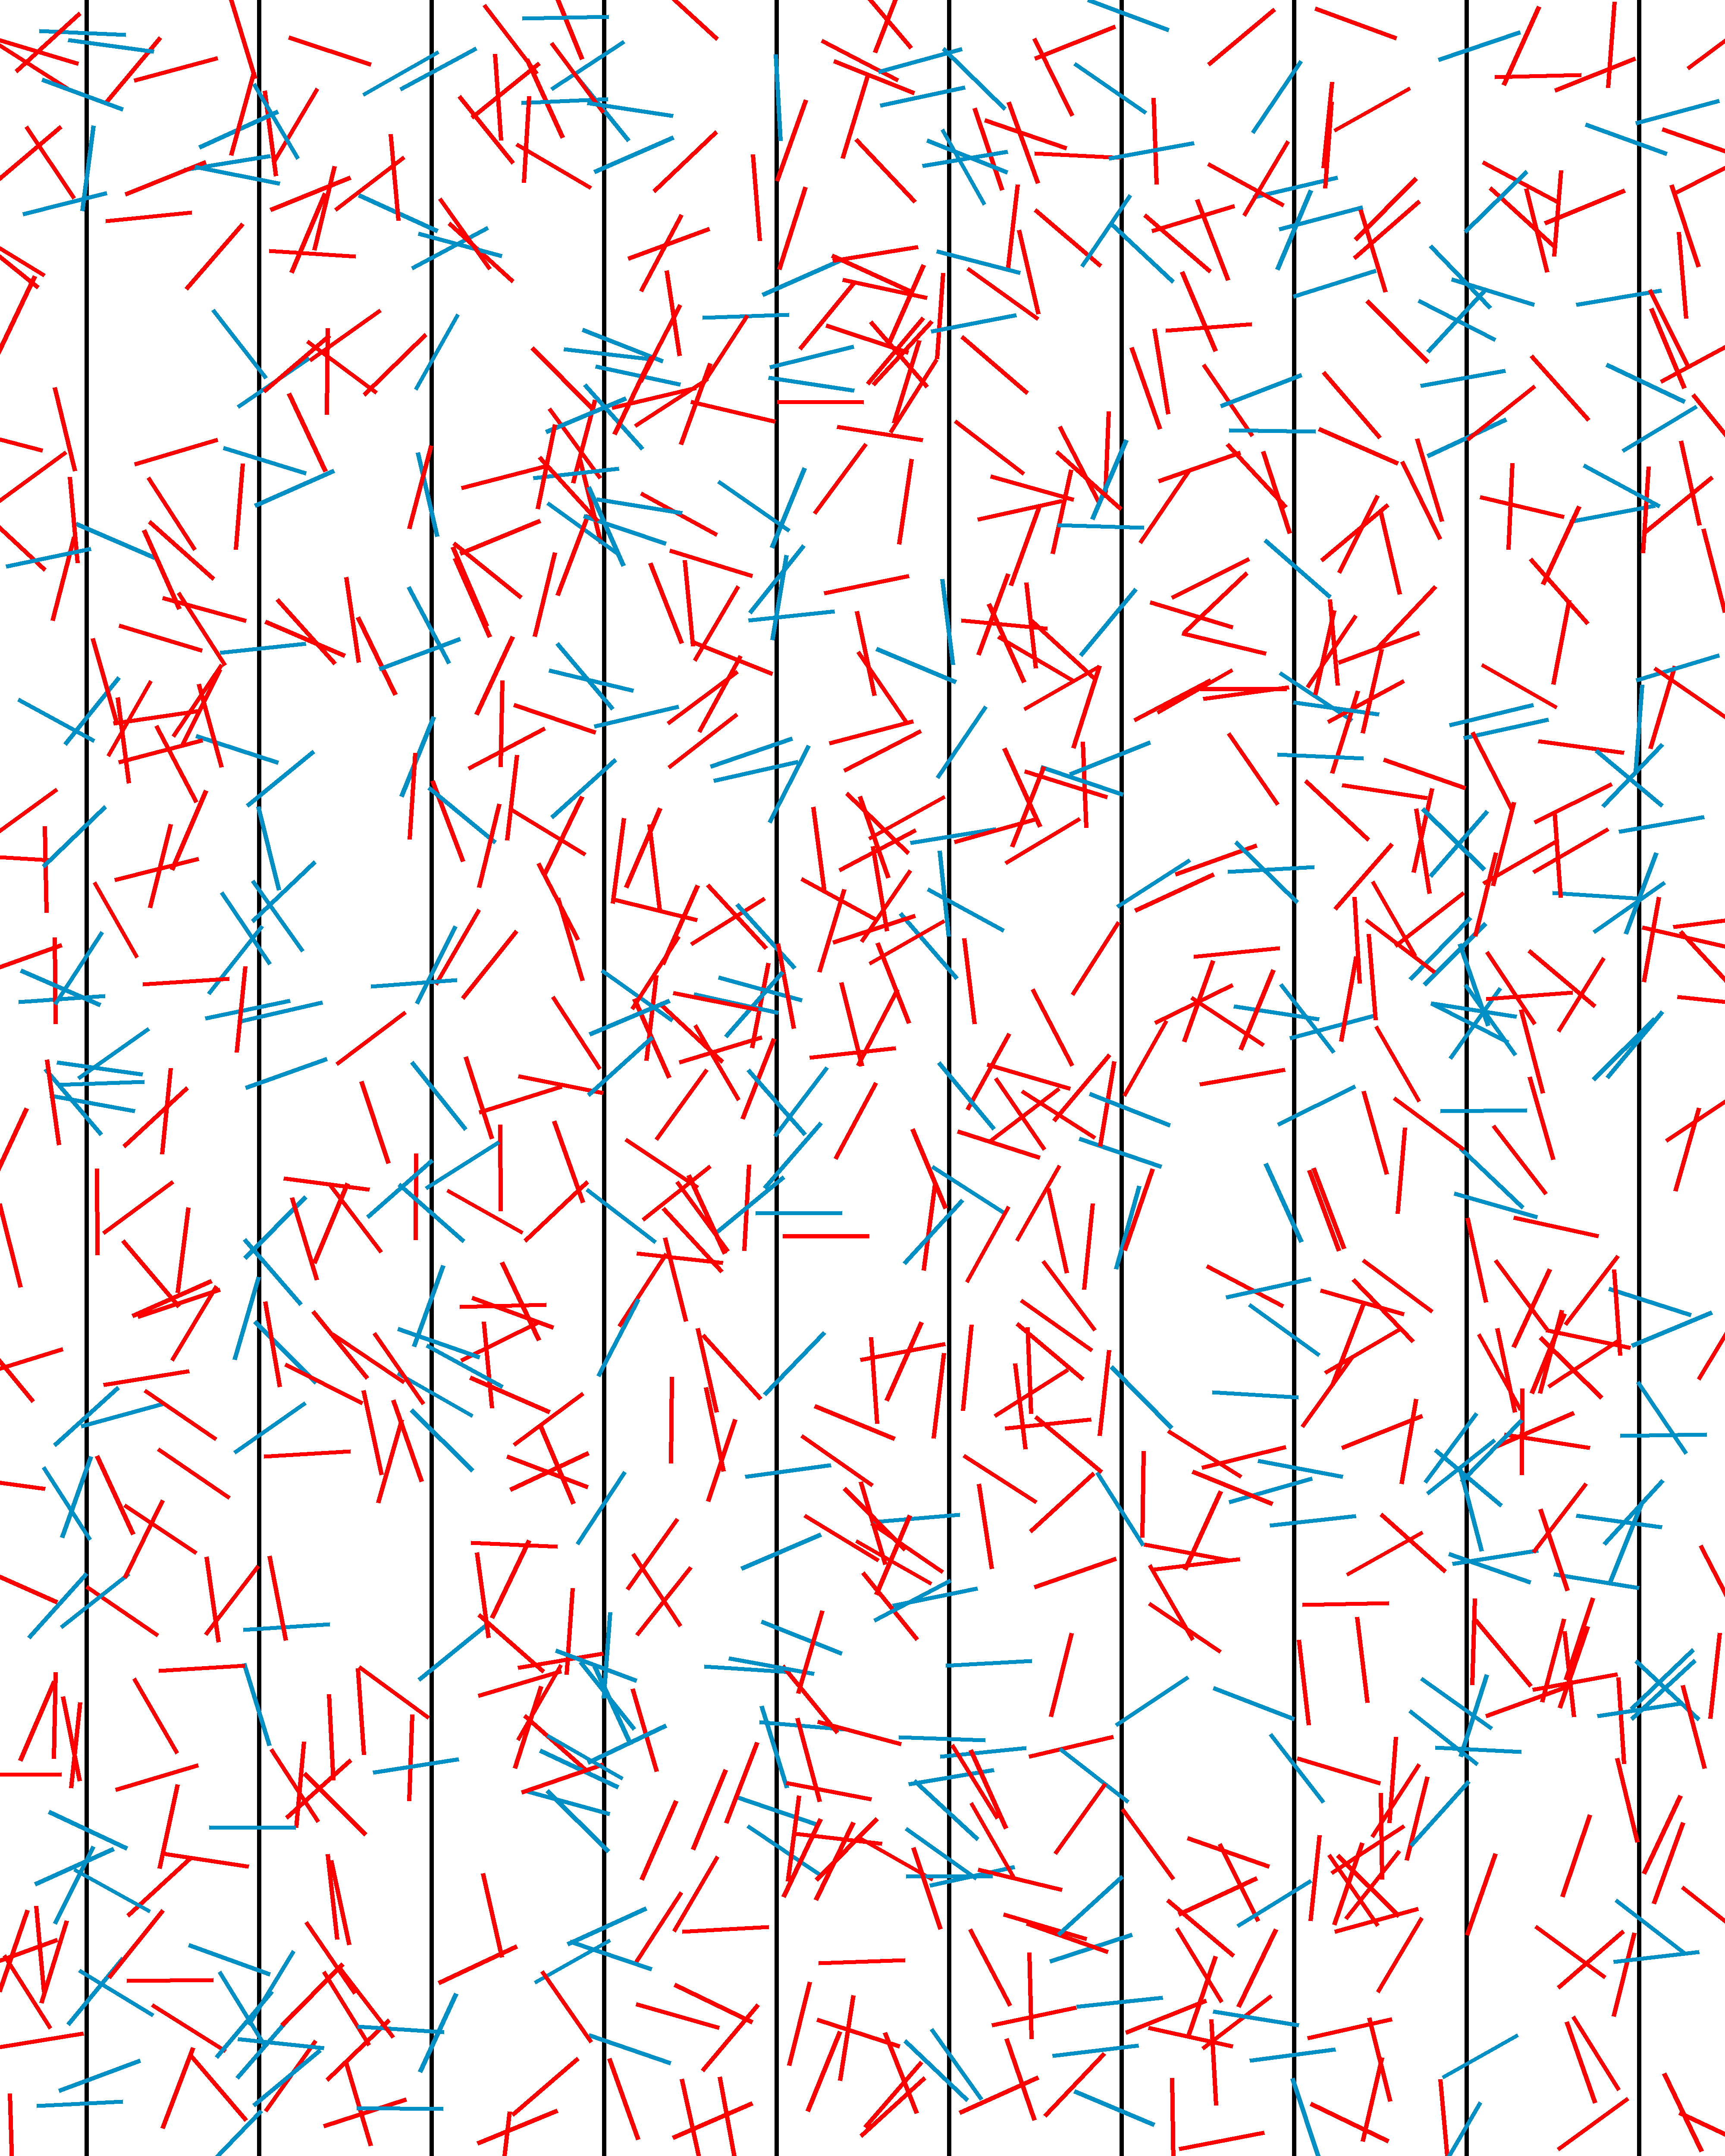
\includegraphics[width=0.45\textwidth]{images/needels.png}
			\caption{Ein Ergebnis der Simulation. Grüne Striche stellen Nadeln dar, die eine Linie schneiden. Rote Striche sind Nadeln, die keine Linie schneiden.}
			\label{fig:needels}
		\end{figure}

		Um zu prüfen, ob eine Nadel eine Linie schneidet, wird der Abstand vom Mittelpunkt der Nadel zur nächsten Linie berechnet. Dann wird mit dem Winkel und der Nadellänge der Abstand in X-Richtung (orthogonal zu den Linien) vom Mittelpunkt der Nadel zur Spitze berechnet. Wenn dieser Abstand größer als der Abstand zur nächsten Linie ist, schneidet die Nadel die Linie:\\
		\texttt{d = (x + line\_dist / 2) \% line\_dist;\\
			dist\_to\_line = min(d, line\_dist - d);\\
			x\_extent = abs(math.cos(angle)) * (needle\_length / 2);\\
			if x\_extent >= dist\_to\_line:}\\
		\\
		Aus dem Ergebnis kann mit der Bibliothek Pillow\cite{Pillow} ein Bild (siehe Abbildung \ref{fig:needels}) erstellt werden, das die geworfenen Nadeln darstellt.

		Für die statistische Auswertung enthält das Programm eine Methode, die Reihe von Simulationen durchführt. Für jede Simulation wird dabei die Anzahl der Nadeln, die eine Linie schneiden, in eine JSON-Datei geschrieben. Diese Datei enthält außerdem die Simulationsparameter, wie die Gesamtanzahl der Nadeln. Dies kann dann im nächsten Schritt ausgewertet werden. So muss die rechenaufwendige Simulation nicht bei jeder Ausführung der andren Module des Programms durchgeführt werden.

	\subsection*{Die Auswertung}
		Es gibt verschiedene Möglichkeiten die Simulationen mit dem Programm auszuwerten. Als erstes kann man aus der JSON-Datei ein Histogramm erzeugen, das die Häufigkeit eines Ergebnisses darstellt. Erstellt werden die Diagramme mit der Bibliothek matplotlib\cite{matplotlib}. Ein Ergebnis ist die Anzahl der Nadeln, die eine Linie schneiden. In Abbildung \ref{fig:hist} sieht man, dass die Ergebnisse normalverteilt sind.

		\begin{figure}[htb]
			\centering
			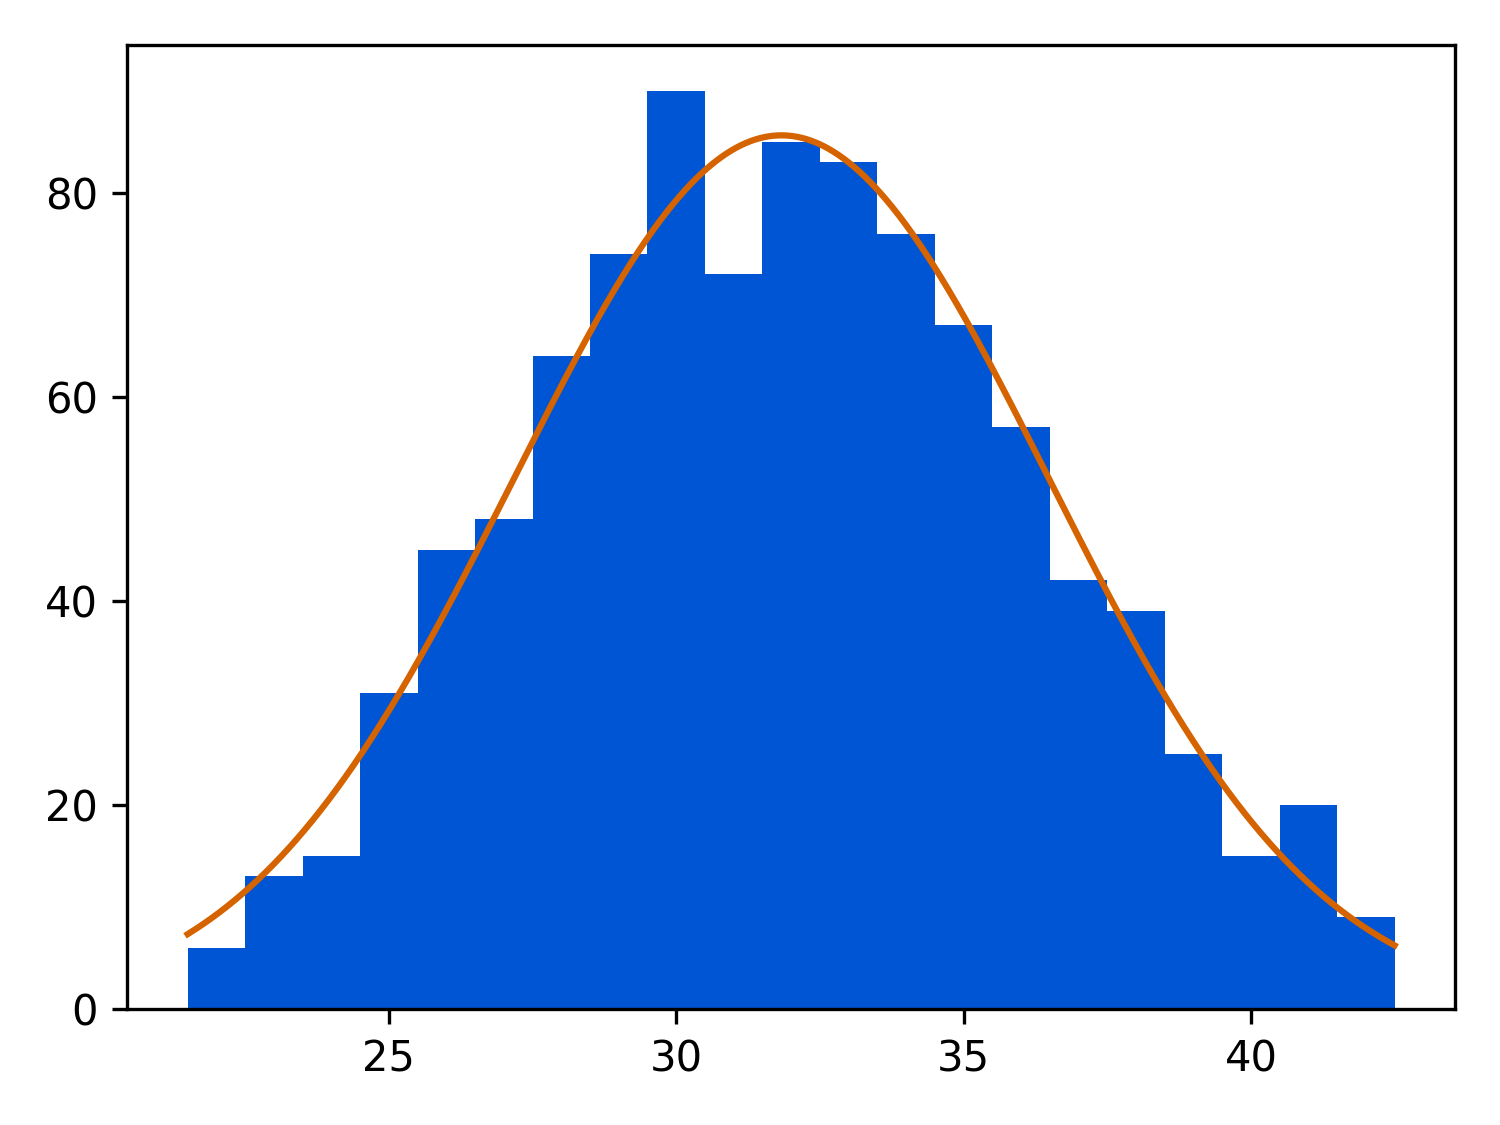
\includegraphics[width=0.45\textwidth]{images/histogram_1000_no_interval_3.png}
			\caption{Histogramm aus 1000 Simulationen mit 100 Nadeln (blau) und Normalverteilung mit gleichen Parametern (orange)}
			\label{fig:hist}
		\end{figure}
		
		Weitere Methoden zur Auswertung werden in den nächsten Kapiteln diskutiert.

\section{Konfidenzintervalle}
	\subsection{Überblick}
		Ein Konfidenzintervall ist ein Bereich, in dem ein bestimmter Parameter mit einer bestimmten Wahrscheinlichkeit liegt. In diesem Kapitel werden Konfidenzintervalle für den Mittelwert $\mu$ und die Varianz $\sigma^2$ untersucht. Diese können verwendet werden um Aussagen über einen unbekannten Parameter der Grundgesamtheit aus den Werten einer Stichprobe treffen zu können.

		In Abbildung \ref{fig_mean_interval_hist} ist das $80\%$ Konfidenzintervall des Mittelwerts dargestellt. In diesem Fall ist das Intervall korrekt, da der wahre Mittelwert, der Hochpunkt der orangen Kurve, innerhalb des Intervalls liegt.
		\begin{figure}[h]%
			\centering
			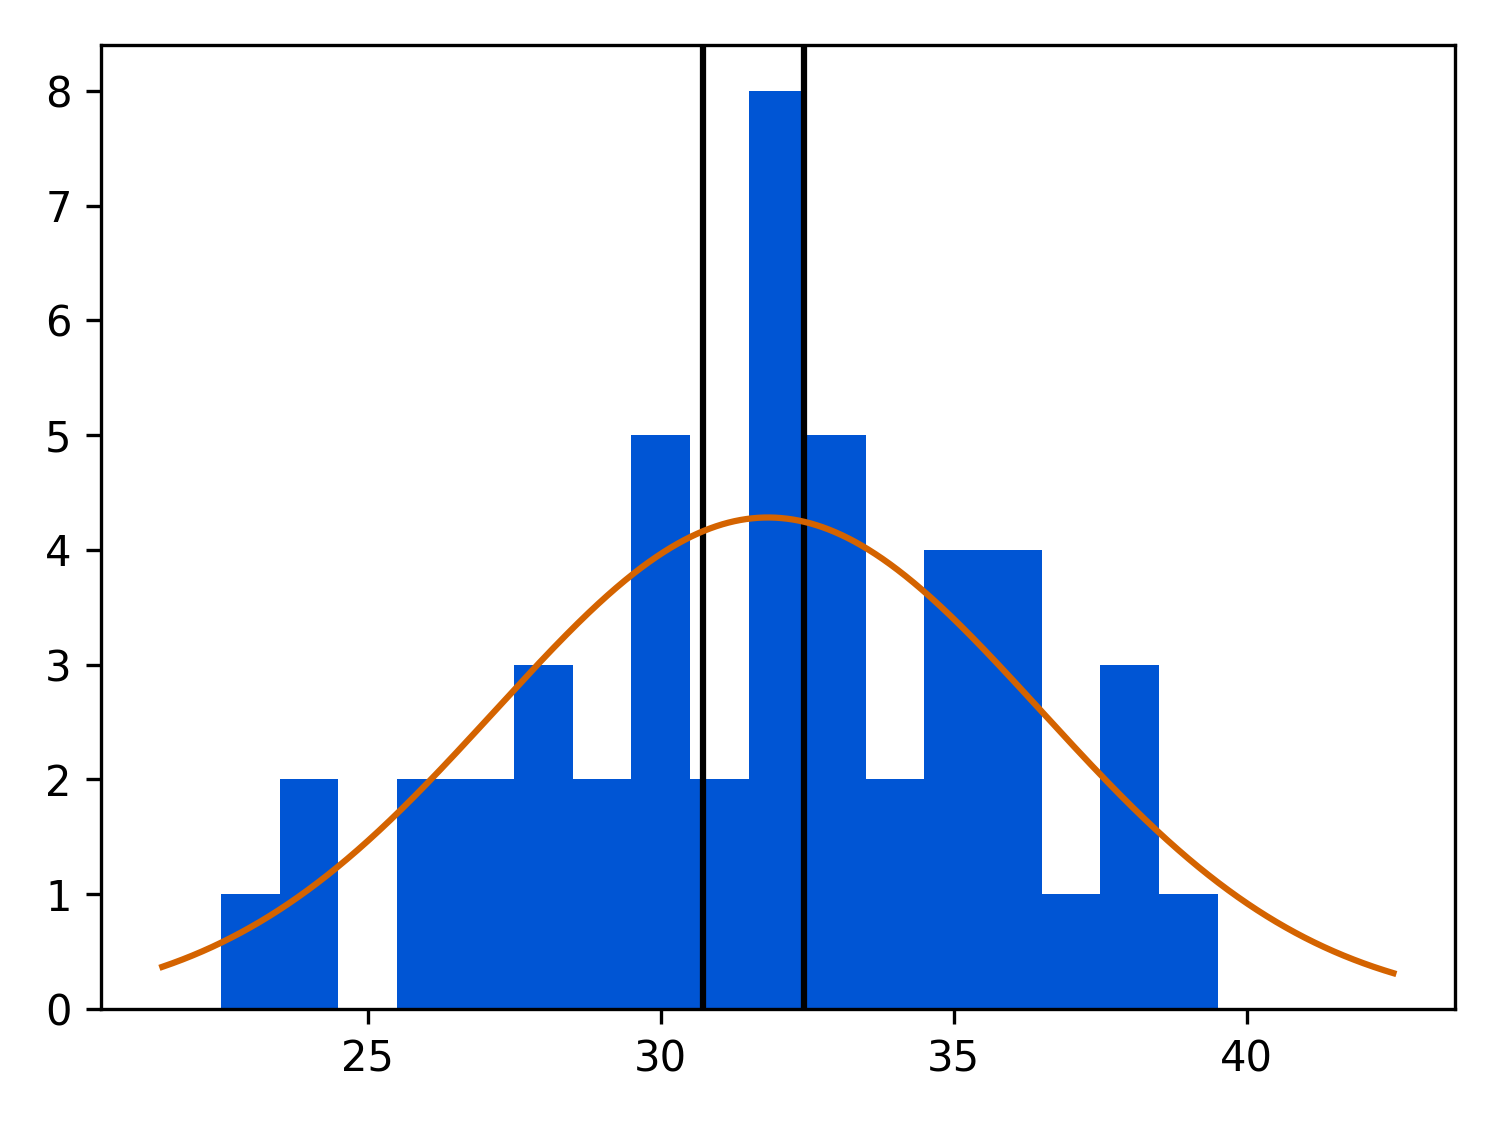
\includegraphics[width=0.9\columnwidth]{images/histogram_50_interval_1.png}
			\caption{Eine Normalverteilung (orange), $50$ nach dieser Verteilung verteilte Werte (blau) und ein aus diesen berechnetes $80\%$ Konfidenzintervall des Mittelwerts (schwarz)}
			\label{fig_mean_interval_hist}
		\end{figure}
	\subsection{Herleitung des Mittelwerts Konfidenzintervalls}
		\label{chap_interval_mean_math}
		Gegeben sind $n$ Stichprobenwerte $x_1, x_2, ..., x_n$ und ein Konfidenzniveau $\gamma$ bzw. eine Irrtumswahrscheinlichkeit $\alpha = 1 - \gamma$.
		Ziel ist die Bestimmung von $c_1$ und $c_2$ sodass
		\begin{equation} \label{eq_interval_norm}
		P(c_1 \le \overline{X} \le c_2) = \gamma
		\end{equation}
		gilt.
		Der Durchschnitt der Stichprobe $\overline{x}$ und die geschätzte Standardabweichung $s$ lasen sich direkt aus den Stichprobenwerten berechnen:
		\begin{align}
		\overline{x} &=  \frac{1}{n} \sum_1^n{x_i} , \\
		s &= \frac{1}{n-1} \sum_1^n{(x_i - \overline{x})^2} .
		\end{align}
		Um Gleichung \ref{eq_interval_norm} umformen zu können wird eine weitere Zufallsvariable eingeführt:
		\begin{equation} \label{eq_interval_t}
		T = \frac{\overline{X} - \mu}{\frac{S}{\sqrt{n}}} .
		\end{equation}
		Gleichung \ref{eq_interval_norm} kann jetzt mit $T$ umformuliert werden:
		\begin{align}
		\gamma &= P(-c \le T \le c) \\ \nonumber
		\gamma &= P(T \le c) - P(T \le -c) \\ \nonumber
		\gamma &= P(T \le c) - (1 - P(T \le c)) \\ \nonumber
		\gamma &= 1 - 2 P(T \le c) \\
		P(T \le c) &= \frac{\gamma + 1}{2} .
		\end{align}
		Da $P(T \le c)$ dem Quantil einer t-Verteilung mit $N = n-1$ Freiheitsgraden entspricht, kann der Wert von $c$ aus einer Tabelle abgelesen werden. Ein genaueres Ergebnis bietet die Funktion \texttt{scipy.stats.t.ppf(x, N)} der Python Bibliothek scipy\cite{scipy}.
		Aus der Definition der Zufallsvariable $T$ in Gleichung \ref{eq_interval_t} ergibt sich für die Grenzen des Intervalls:
		\begin{equation}
		c_1 = \overline{x} - \frac{cs}{\sqrt{n}} \mbox{ und } c_2 = \overline{x} + \frac{cs}{\sqrt{n}}.
		\end{equation}

	\subsection{Herleitung des Varianz Konfidenzintervalls}
		\label{chap_interval_var_math}
		Die Herleitung des Varianz Intervalls verläuft analog zu dem Konfidenzintervall  des Mittelwerts. Anstelle einer t-Verteilung wird eine Chi-Quadrat-verteilte Zufallsvariable eingeführt:
		\begin{equation} \label{eq_interval_z}
		Z = (n-1)\frac{S^2}{\sigma^2} .
		\end{equation}
		\begin{align}
		\gamma &= P(c_1 \le Z \le c_2) \\
		\gamma &= P(Z \le c_2) - P(Z \le c_1) \nonumber \\
		P(Z \le c_1) &= \frac{1}{2} (1-\gamma) \\
		P(Z \le c_2) &= \frac{1}{2} (1+\gamma)
		\end{align}
		$P(T \le c_{1,2})$ entspricht jeweils einem Quantil einer Chi-Quadrat-Verteilung mit $N = n-1$ Freiheitsgraden, dies kann durch \texttt{scipy.stats.chi2.ppf(x, N)}\cite{scipy} berechnet werden.
		Aus der Definition der Zufallsvariable $Z$ in Gleichung \ref{eq_interval_z} ergibt sich das Konfidenzintervall der Varianz:
		\begin{equation}
		(n-1)  \frac{s^2}{c_2} \le \sigma^2 \le (n-1)  \frac{s^2}{c_1}.
		\end{equation}

	\subsection{Empirischer Beweis}
		\label{chap_interval_prove}
		Insbesondere durch die Annahmen, die in Gleichung \ref{eq_interval_t} und \ref{eq_interval_z} eingeführte  Zufallsvariablen $T$ und $Z$ würde genau einer t-Verteilung bzw. Chi-Quadrat-Verteilung mit jeweils $N = n-1$ Freiheitsgraden entsprechen, ist die Herleitung alleine nur bedingt geeignet um die daraus gewonnen Formeln zu plausibilisieren.

		Um die Korrektheit der in Kapitel \ref{chap_interval_mean_math} hergeleiteten Formeln zu bestätigen wurde ein empirischer Beweis durchgeführt. Die Berechnung wurde in Python implementiert und können so beliebig oft mit den in Kapitel \ref{chap_sim_results} erstellten Daten durchgeführt werden.

		Der folgende Test wird separat für mehrere Werte von $\gamma \in [0, 1]$ durchgeführt. Es wird für $n = 20$ Werte das Konfidenzintervall des Mittelwerts und der Varianz mit einem Konfidenzniveau $\gamma$ gebildet. Durch den in Kapitel \ref{chap_buffon_needle} hergeleiteten Wert für $p$ können der theoretisch zu erwartenden Mittelwerts und die Varianz berechnet  werden:
		\begin{align}
		E(X) &= n p , \\
		\sigma &= n p (1-p) , \nonumber \\
		Var(X) &= \sigma^2 = (n p (1-p))^2 .
		\end{align}

		Es wird überprüft, ob der Erwartungswert und die Varianz innerhalb oder außerhalb des geschätzten Intervalls liegen.

		Dieser Vorgang wird in $10^5$ Durchläufen wiederholt, dabei wird der Anteil an korrekten Intervalle gezählt. Daraus wird das Verhältnis zwischen dem tatsächlichen Anteil an korrekten Intervallen und $\gamma$ berechnet, wenn die Formeln stimmen ist der Erwartungswert dieses Verhältnisses $1$.

		Um zu zeigen, dass diese Methode der Überprüfung funktioniert wurde nicht nur die hergeleiteten Formeln, sondern auch absichtlich falsche Formeln überprüft. Für die falschen Formeln wurden $n$ Freiheitsgrade angenommen (richtig sind $n-1$). Abhängig von den Parametern ist dieser Fehler schwer zu erkennen, da die Ergebnisse liegen sehr nahe an den eigentlich richtigen liegen.

		Die Ergebnisse sind in Abbildung \ref{fig_mean_interval_dot} und \ref{fig_var_interval_dot} dargestellt. Dabei ist klar zu erkennen, dass die mit den richtigen Formeln berechneten Ergebnisse nahe an $1$ liegen und die mit den falschen Formeln berechneten Ergebnisse deutlich von $1$ abweichen. Dies bestätigt die Korrektheit der Formeln und des Testverfahrens.

		\begin{figure}[H]%
			\centering
			\begin{subfigure}[c]{1\columnwidth}
				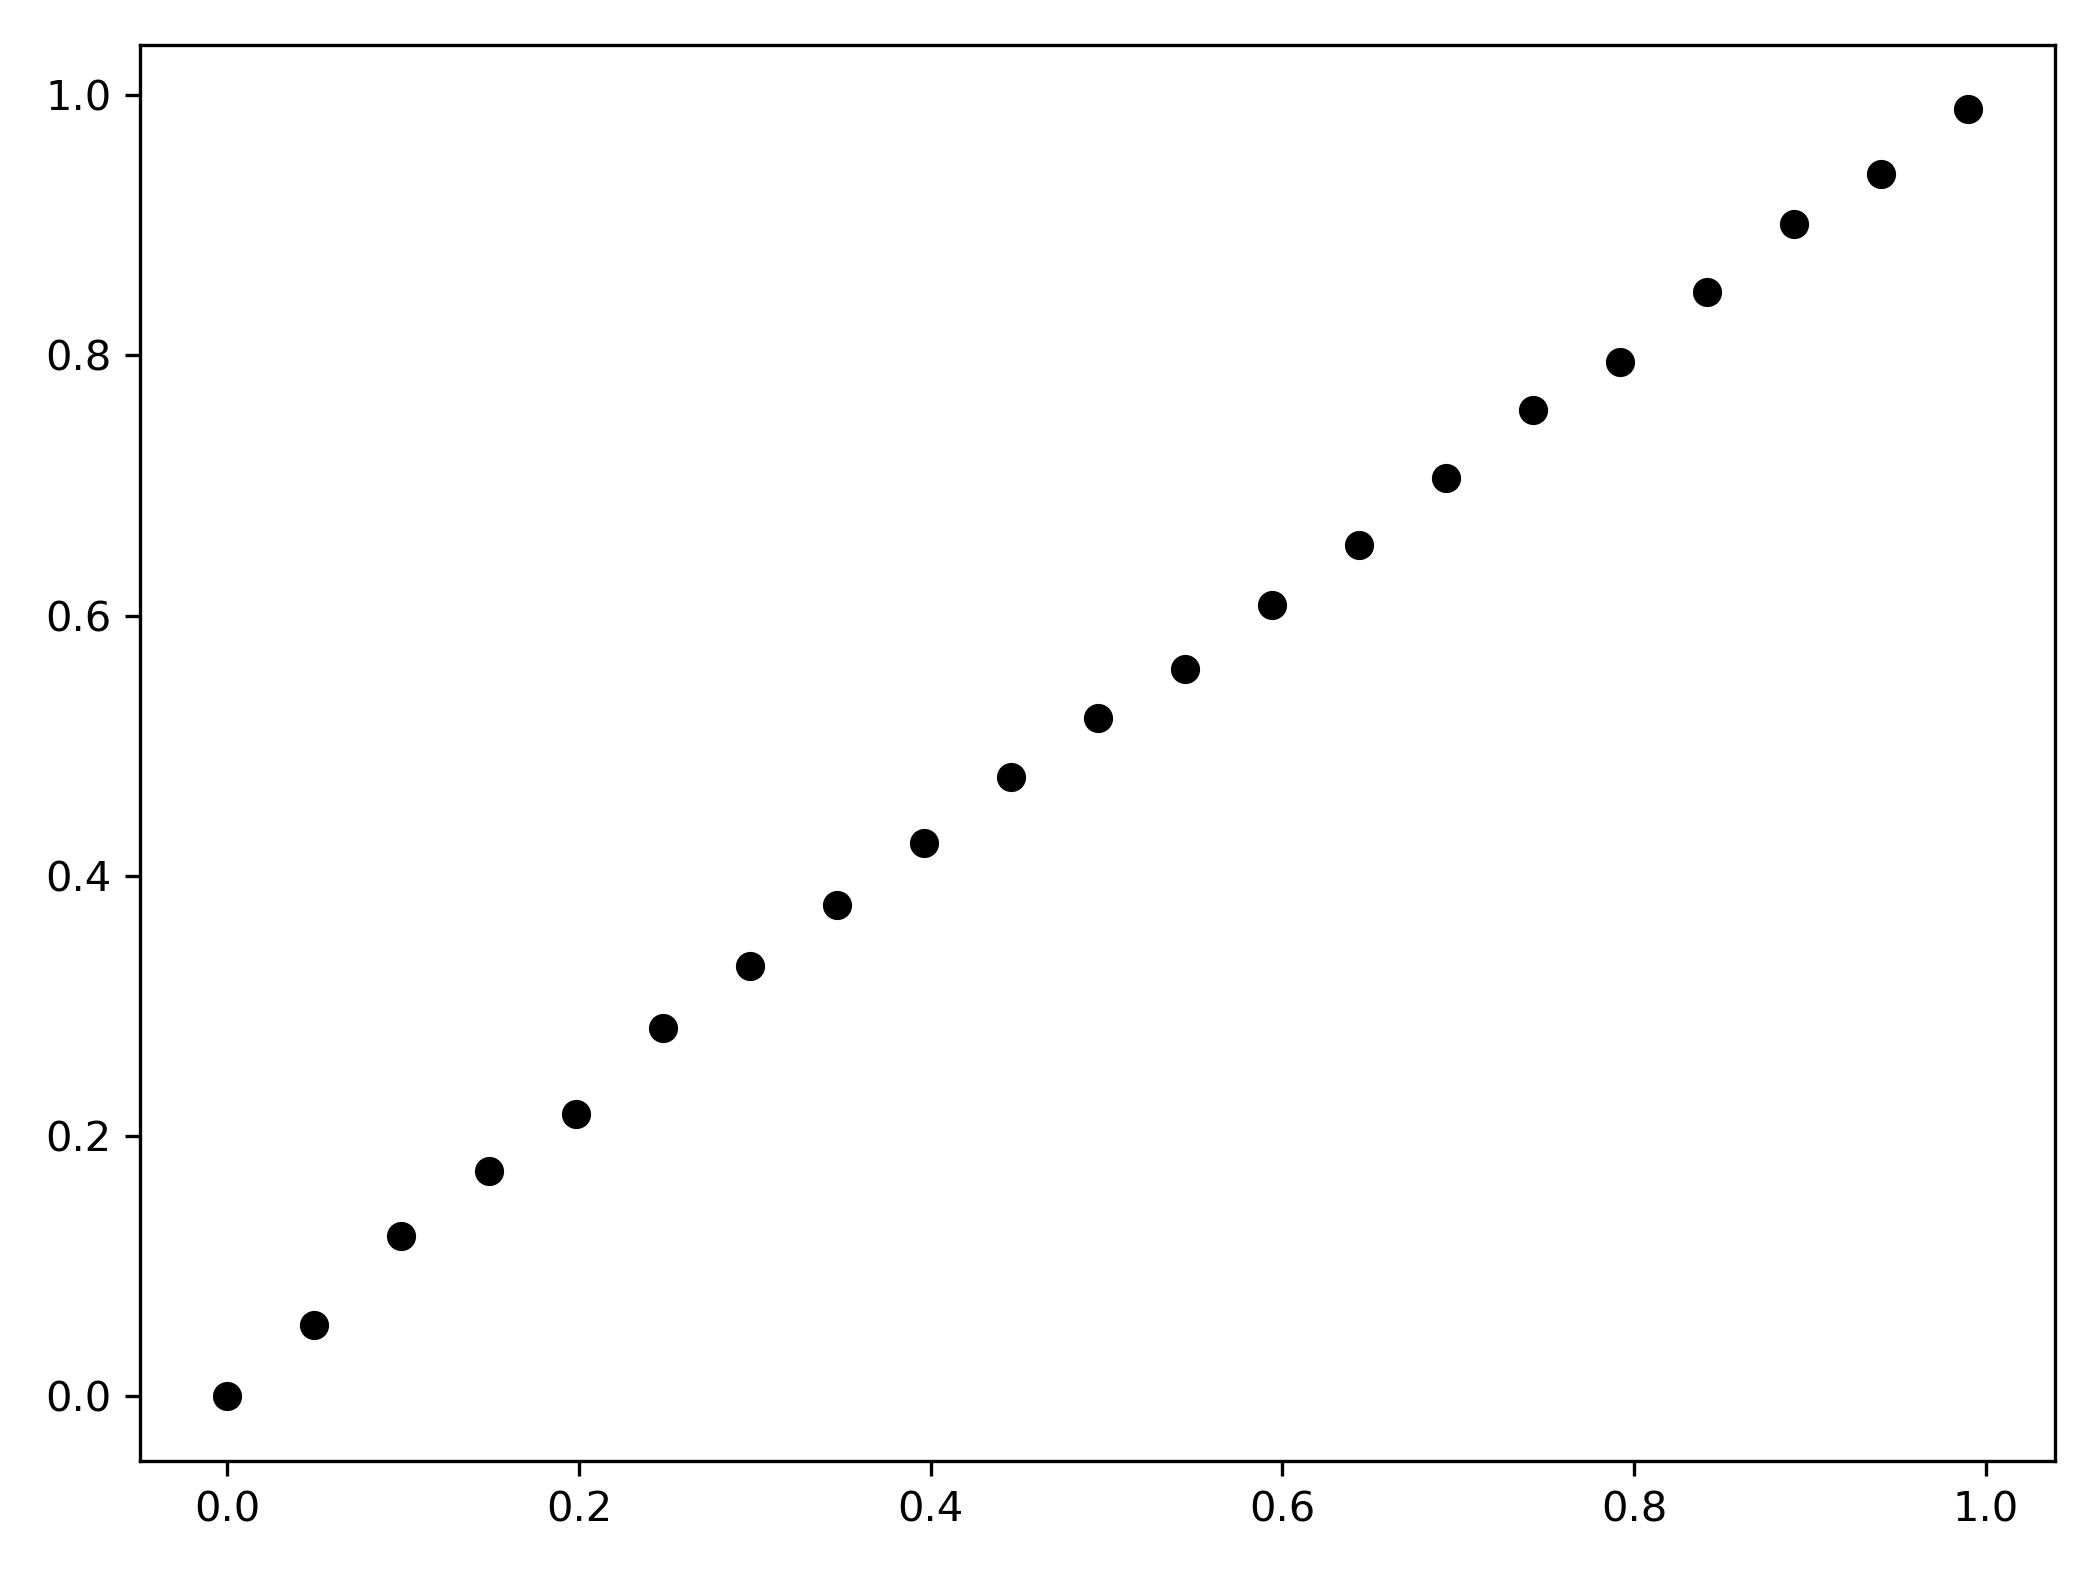
\includegraphics[width=0.9\columnwidth]{images/mean_interval.png}
				\caption{Mittelwerts Konfidenzintervall}
				\label{fig_mean_interval_dot}
			\end{subfigure}
			\begin{subfigure}[c]{1\columnwidth}
				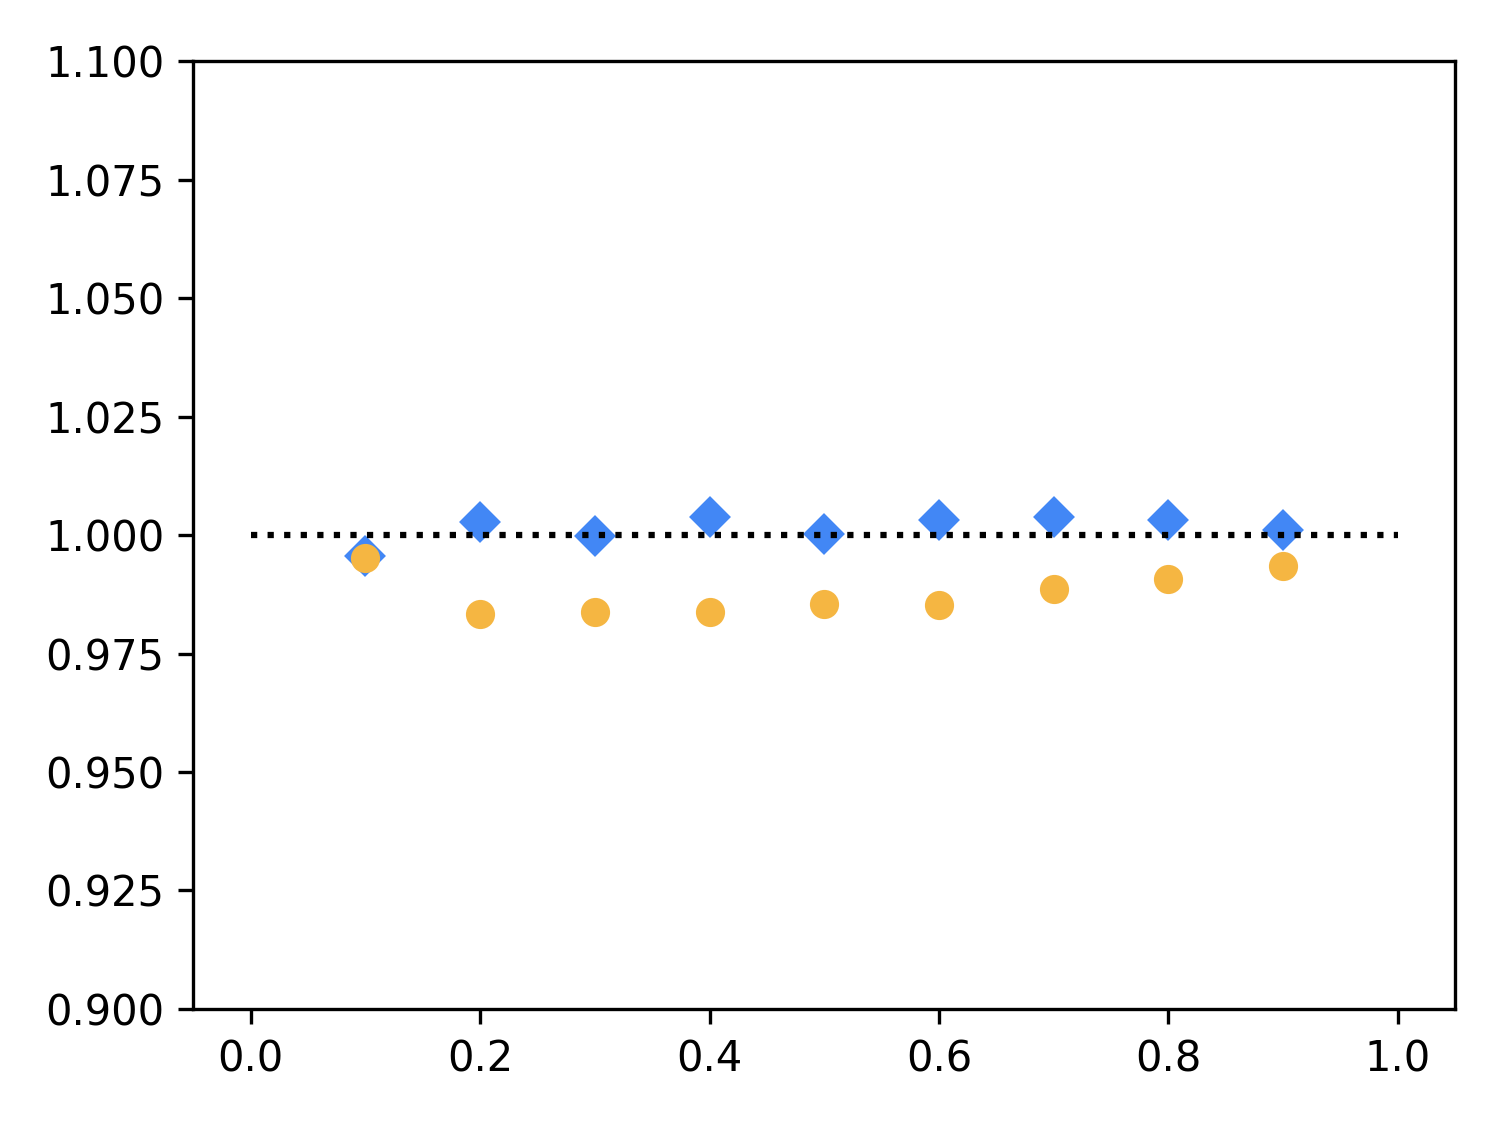
\includegraphics[width=0.9\columnwidth]{images/var_interval.png}
				\caption{Varianz Konfidenzintervall}
				\label{fig_var_interval_dot}
			\end{subfigure}
			\caption{Abweichung des tatsächlichen Anteils an korrekt geschätzten Intervallen von dem Konfidenzniveau (y-Achse) für verschiedene Konfidenzniveaus (x-Achse) von dem idealen Wert (schwarz) für Ergebnisse der richtigen Formeln (blau) und der falschen Formeln (gelb).}
		\end{figure}


\section{Parametertests}
	\subsection{Überblick}
		Mit einem Parametertest kann eine Aussage darüber gemacht werden, ob ein bestimmter Wert eines Parameters angesichts der bekannten Werten einer Stichprobe plausibel ist. In diesem Kapitel werden Konfidenzintervalle für den Mittelwert $\mu$ untersucht. Dieser kann beispielsweise verwendet werden um Angaben eines Herstellers zu überprüfen.
	\subsection{Herleitung des Mittelwerts Parametertests}
		Gegeben sind $n$ Stichprobenwerte $x_1, x_2, ..., x_n$ und ein Konfidenzniveau $\gamma$ bzw. eine Irrtumswahrscheinlichkeit $\alpha = 1 - \gamma$. Es soll getestet werden, ob ein angegebener Wert des Mittelwerts der Grundgesamtheit $\mu_0$ korrekt ist.

		Das Ziel ist die Entscheidung zwischen einer Nullhypothese $H_0$ ($\mu = \mu_0$) und einer Alternativhypothese $H_1$ ($\mu \ne \mu_0$).

		Das Vorgehen ähnelt dem Schätzen eines Mittelwerts Konfidenzintervalls. Es wird die Zufallsvariable $T$ eingeführt (Gleichung \ref{eq_interval_t}), mit dieser kann der Test formuliert werden als:
		\begin{equation}
		P(-c \le T \le c) = \gamma .
		\end{equation}
		$c$ wird wieder aus den Quantilen der t-Verteilung berechnet. Es wird aber $c$ nicht aus $T$ in $X$ rücktransformiert um die Grenzen des Konfidenzintervalls zu erhalten, sondern der Mittelwert der Stichprobe wird nach $T$ transformiert:
		\begin{equation}
		\hat{t} = \frac{\overline{x} - \mu_0}{\frac{s}{\sqrt{n}}} .
		\end{equation}

		Dann gilt mit einer Wahrscheinlichkeit $\gamma$, dass $H_0$ wahr ist, wenn
		\begin{equation}
		-c \le \hat{t} \le c
		\end{equation}
		gilt, andernfalls ist $H_1$ wahr.

		Mit einer höheren Irrtumswahrscheinlichkeit $\alpha = 1 - \gamma$ sinkt die Wahrscheinlichkeit $H_0$ fälschlich abzulehnen, dafür steigt die Wahrscheinlichkeit $H_0$ fälschlich anzunehmen.
	\subsection{Empirischer Beweis}
		Das die hergeleiteten Formeln gelten ist auch hier nicht sofort plausibel.

		Das Vorgehen entspricht im Wesentlichen dem aus Kapitel \ref{chap_interval_prove}. Die Auswertung gestaltet sich etwas einfacher, da der Parametertest direkt einen Wahrheitswert liefert, die Annahme oder Ablehnung von $H_0$.

		Die Ergebnisse sind in Abbildung \ref{fig_test_mean_dot} zu sehen. Die Ergebnisse der richtigen Formeln liegen wieder nahe an $1$ und die der falschen Formeln weichen deutlich von $1$ ab. Dies bestätigt die Korrektheit der Formeln und des Testverfahrens.

		\begin{figure}[H]
			\centering
			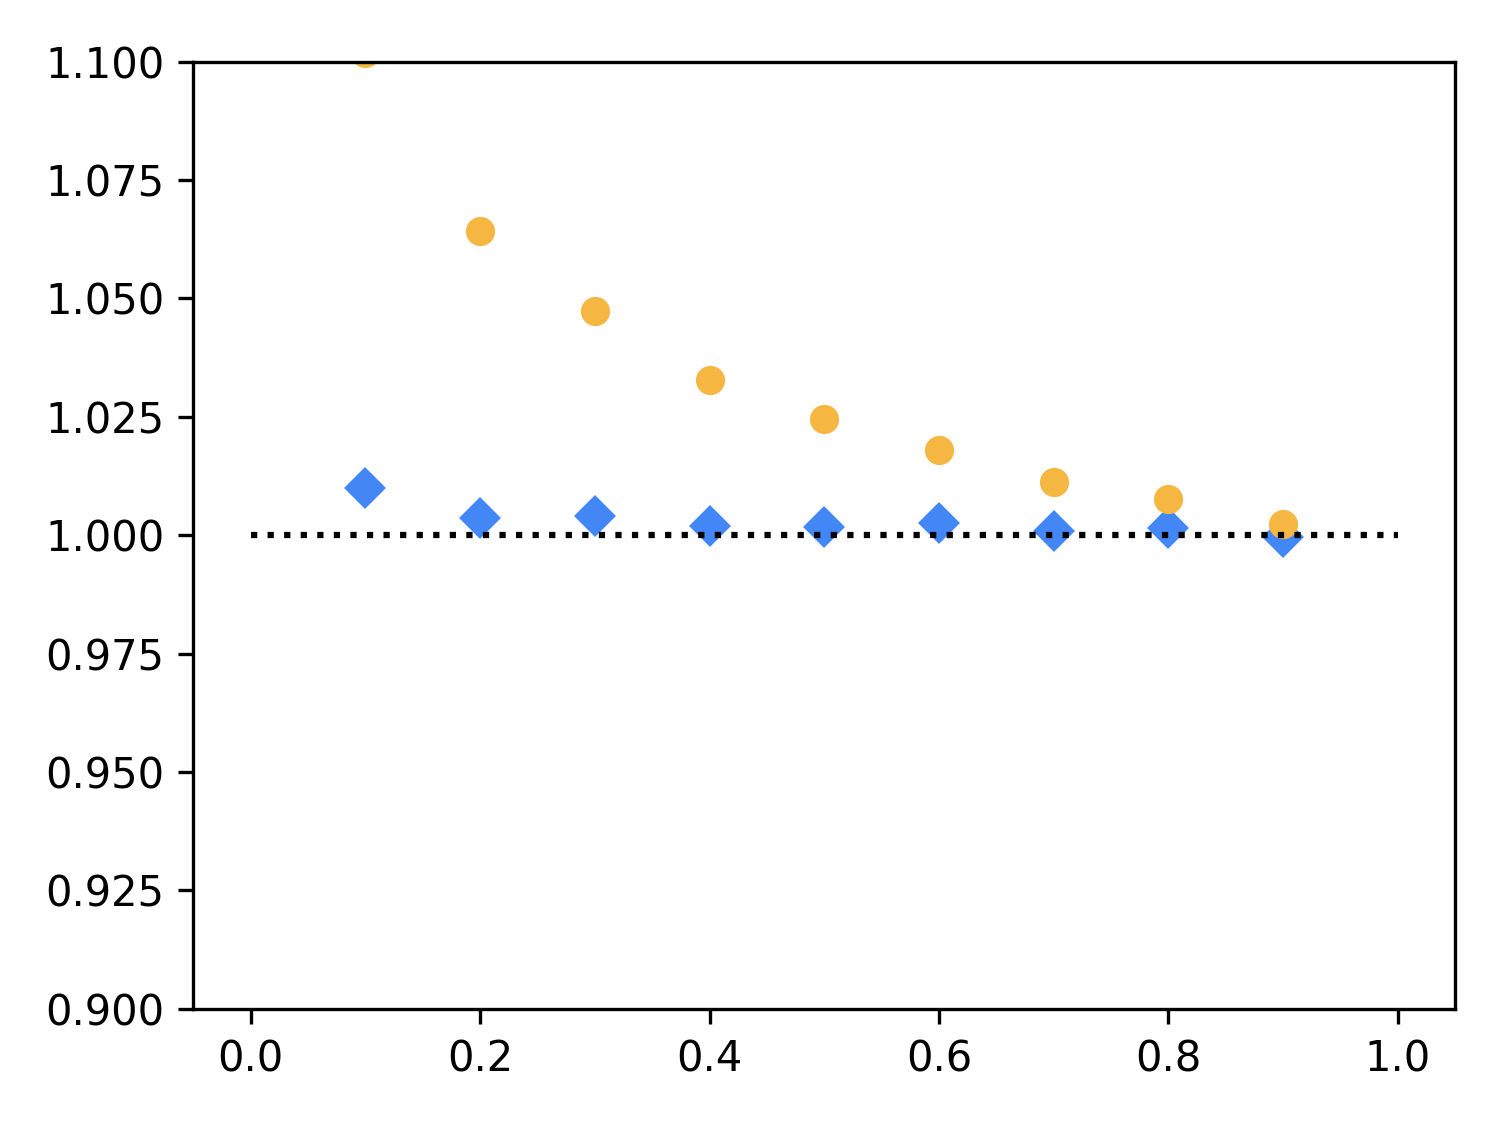
\includegraphics[width=0.9\columnwidth]{images/mean_test.png}
			\caption{Abweichung des Anteils negativer Parametertests von der Irrtumswahrscheinlichkeit (y-Achse) für verschiedene Irrtumswahrscheinlichkeiten (x-Achse) von dem idealen Wert (schwarz) für Ergebnisse der richtigen Formeln (blau) und der falschen Formeln (gelb).}
			\label{fig_test_mean_dot}
		\end{figure}

\section{Experimenteller Test von Lazzarini}
	Es gab mehrere Versuche durch eine praktische Durchführung des Buffonschen Nadelexperiments den Wert für $\pi$ anzunähern. Mario Lazzarini soll 1901 das umfangreichste Experiment durchgeführt haben. Hierfür baute er eigens eine Maschine und führte das Experiment mit 3408 Nadelwürfen durch. Das Längenverhältnis betrug hierbei ${\tfrac {l}{d}={\tfrac {5}{6}}}$. Mit einem Ergebnis von 1808 Nadeln, die eine Linie schneiden, schaffte Lazzarini es mit diesem Experiment den Wert von $\pi$ auf 6 Nachkommastellen anzunähern. Diese hohe Genauigkeit wurde von vielen als Glückstreffer oder Fälschung gesehen.\cite{Badger}

	Wie glaubwürdig Lazzarinis Ergebnis war, lässt sich mit Hilfe eines Konfidenzintervalls bestimmen. Hierbei wird die Genauigkeit wie folgt berechnet:
	\begin{equation}
	\Delta \mu = c_2 - \overline{x} = \frac{cs}{\sqrt{n}}
	\end{equation}
	In Lazzarinis Versuch beträgt die Standartabweichung $s = 0.249141$.
	Für ein Konfidenzniveau von $\gamma = 0.95$ ergibt sich folgende Gleichung:
	\begin{equation}
	P(T \le c) = \frac{\gamma + 1}{2} = \frac{0.95 + 1}{2} = 0.975
	\end{equation}
	Mit $N = n - 1 = 3407$ Freiheitsgraden erhält man $c = 1,96066$.
	Somit erreichte Lazzarini bei seinem Experiment eine Genauigkeit von
	\begin{align}
	\Delta \mu &= \frac{cs}{\sqrt{n}} \\
	&= \frac{1,96066 \cdot 0.249141}{\sqrt{3408}} \\ \nonumber
	&= 8,367538 \cdot 10 ^{-3} \nonumber
	\end{align}
	für den Mittelwert. Die Genauigkeit für den $\pi$ Wert ist dann:
	\begin{align}
	\Delta x &= \pi - \frac{2 \cdot x}{P + \Delta \mu} \\
	&= \pi - \frac{2 \cdot \frac{5}{6}}{\frac{1808}{3408} + 8,367538 \cdot 10 ^{-3}} \\ \nonumber
	&= 0.048781 \nonumber
	\end{align}
	Das ist deutlich ungenauer als $\Delta x = 0,5 * 10^{-6}$, was 6 Nachkommastellen entsprechen würde.
	Also ist der ermittelte Wert für $\pi$ von Lazzarini ab der zweiten Nachkommastelle bedeutungslos.
	
\section*{Ergebnisse und Diskussion}

\begin{thebibliography}{99}
	\bibitem{MathWorld}Weisstein, Eric W.: {\textit Buffon's Needle Problem.}, From MathWorld--A Wolfram Web Resource. \url{https://mathworld.wolfram.com/BuffonsNeedleProblem.html}
	\bibitem{Python}Python: \url{https://www.python.org/}
	\bibitem{Pillow}Pillow: \url{https://pillow.readthedocs.io/en/stable/}
	\bibitem{matplotlib}matplotlib: \url{https://matplotlib.org/}
	\bibitem{scipy}scipy: \url{https://www.scipy.org/}
	\bibitem{Badger}Lee Badger: Lazzarini’s Lucky Approximation of $\pi$, Mathematics Magazine, Band 67, 1994, 83-85
\end{thebibliography}

\end{document}